\documentclass{beamer}

\mode<presentation>
{
\usetheme{Copenhagen}
%\usetheme{Boadilla}
%\usecolortheme{seahorse}
%\useoutertheme{infolines}
%\useoutertheme[compress]{miniframes}
%\setbeamercovered{transparent}
}

%% \mode<presentation>
%% {
%% \usetheme{progressbar}
%% \setbeamercovered{transparent}
%% }

%\usepackage[english]{babel}
\usepackage[english]{babel}
\usepackage[utf8]{inputenc}
\usepackage[T1]{fontenc}

\usepackage{mathptmx}
\usepackage[scaled=.90]{helvet}
\usepackage[T1]{fontenc}
\usepackage{xspace}
%\usepackage{appendixnumberbeamer}
\usepackage[noend]{algorithmic}
%\usepackage[algo2e,vlined,algochapter,ruled,dotocloa]{algorithm2e}
\usepackage{fancybox}
\usepackage{algorithm}
\usepackage[noend]{algorithmic}
\usepackage{amssymb,amsmath}
% \usepackage{ulem}
\usepackage{makecell}
\usepackage{times}
\usepackage{bbding}

\title[A few topics in Reinforcement Learning]{From Field problems to Machine Learning}
\subtitle{An introduction to the Data Science workflow\\and a motivation to understand Machine Learning}
%\title{The Optimal Swapping Problem during Nuclear Refueling Operations}


\author{E. Rachelson}

\institute{
\includegraphics[width=1.5cm]{img/isae.jpg}}

\date{}

\setbeamerfont{bibliography entry author}{shape=\upshape,series=\bfseries,size=\footnotesize}%
\setbeamerfont{bibliography entry title}{shape=\upshape,size=\scriptsize,series=\mdseries}
\setbeamerfont{bibliography entry journal}{shape=\upshape,size=\scriptsize,series=\mdseries}
\setbeamerfont{bibliography entry note}{shape=\upshape,size=\scriptsize,series=\mdseries}

\setbeamercolor{block}{bg=blue,fg=red}

\beamertemplatenavigationsymbolsempty
\setbeamertemplate{footline}[frame number]

\begin{document}


\begin{frame}{Artificial Neural Networks}
Keywords:
\begin{itemize}
\item Computation graph $f_\theta(x)$
\item Forward pass and gradient backpropagation
\item Online training
\item Minibatches
\item The vanishing gradient problem
\item Keras, Tensorflow, Caffe, Pytorch, Theano
\item Avoiding overfitting: dropout, regularization, data augmentation
\item Convolutional neural networks
\end{itemize}
\end{frame}

\begin{frame}{Artificial Neural Networks}
\begin{itemize}
\item Versatile, online training
\item State-of-the-art performance on many benchmarks
\item But fragile and hard to tune
\item Lots of "recipes" still today
\item Hard to guarantee convergence or performance
\item CNNs = method of choice for structured data (images, sound, time series\ldots)
\end{itemize}
\begin{center}
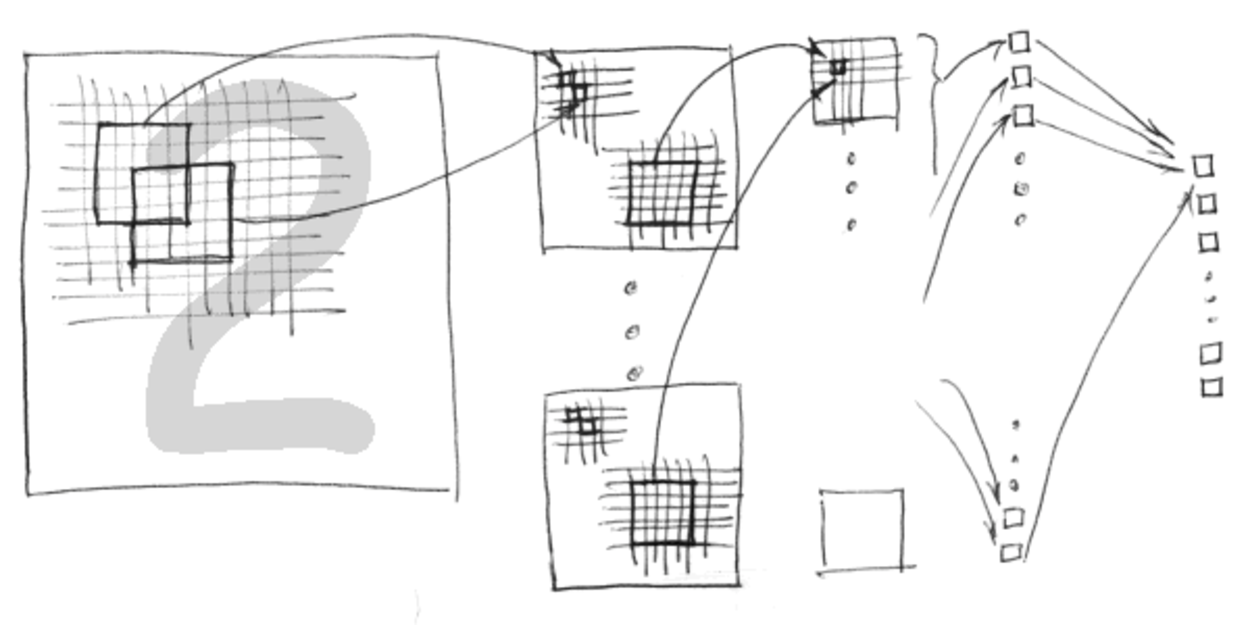
\includegraphics[width=7cm]{img/IllustrationNeuralNet.pdf}
\end{center}
\end{frame}

\end{document}
